\chapter{Decision Frameworks: When to Use What}
\label{chap:decision_frameworks}

\begin{tldr}
This chapter provides decision frameworks for architecture selection, loss function choice, model sizing, and common trade-offs. Staff-level interviews often test whether you can make principled decisions given constraints—not just whether you know techniques. These frameworks encode best practices and help structure your thinking during system design questions.
\end{tldr}

\section{Architecture Selection}
\label{sec:arch_selection}

\subsection{By Data Modality}

\begin{figure}[H]
\centering
\begin{tikzpicture}[
    node distance=0.8cm,
    decision/.style={diamond, draw, aspect=2, inner sep=1pt, fill=yellow!20, font=\small},
    result/.style={rectangle, draw, rounded corners, fill=lightgreen, minimum width=2.5cm, font=\small, align=center},
    arrow/.style={->, thick}
]
    \node[decision] (modality) {Data modality?};
    
    % Branches
    \node[result, below left=1.5cm and 2.5cm of modality] (tabular) {Gradient Boosting\\(XGBoost, LightGBM)};
    \node[result, below left=1.5cm and 0cm of modality] (image) {CNN / ViT};
    \node[result, below right=1.5cm and 0cm of modality] (text) {Transformer};
    \node[result, below right=1.5cm and 2.5cm of modality] (graph) {GNN};
    
    % Edges
    \draw[arrow] (modality) -- node[above, font=\tiny, sloped] {Tabular} (tabular);
    \draw[arrow] (modality) -- node[above, font=\tiny, sloped] {Image} (image);
    \draw[arrow] (modality) -- node[above, font=\tiny, sloped] {Text/Seq} (text);
    \draw[arrow] (modality) -- node[above, font=\tiny, sloped] {Graph} (graph);
    
    % Sub-decisions for images
    \node[decision, below=1cm of image] (imgdata) {Data size?};
    \node[result, below left=0.8cm and 0cm of imgdata, minimum width=1.5cm] (cnn) {CNN};
    \node[result, below right=0.8cm and 0cm of imgdata, minimum width=1.5cm] (vit) {ViT};
    
    \draw[arrow] (image) -- (imgdata);
    \draw[arrow] (imgdata) -- node[left, font=\tiny] {Small} (cnn);
    \draw[arrow] (imgdata) -- node[right, font=\tiny] {Large} (vit);
\end{tikzpicture}
\caption{Architecture selection by data modality.}
\label{fig:arch_by_modality}
\end{figure}

\subsection{Comprehensive Architecture Decision Table}

\begin{table}[H]
\centering
\caption{Architecture selection by task and constraints}
\begin{tabularx}{\textwidth}{lXXX}
\toprule
\textbf{Task} & \textbf{First Choice} & \textbf{Alternative} & \textbf{When to Choose Alt} \\
\midrule
\multicolumn{4}{l}{\textbf{Tabular Data}} \\
Classification/Regression & XGBoost/LightGBM & Neural network & Deep interactions needed \\
Time series & LightGBM + features & Transformer, LSTM & Long-range patterns \\
\midrule
\multicolumn{4}{l}{\textbf{Images}} \\
Classification (small data) & ResNet, EfficientNet & — & — \\
Classification (large data) & ViT, Swin & ConvNeXt & Less compute \\
Detection & YOLO, DETR & Faster R-CNN & Accuracy over speed \\
Segmentation & U-Net, DeepLab & Mask R-CNN & Instance segmentation \\
\midrule
\multicolumn{4}{l}{\textbf{Text}} \\
Classification & BERT, RoBERTa & DeBERTa & SOTA needed \\
Generation & GPT, LLaMA & — & — \\
Translation/Summarization & T5, BART & LLM few-shot & No training data \\
\midrule
\multicolumn{4}{l}{\textbf{Retrieval}} \\
< 10K items & Cross-Encoder & — & — \\
10K - 1M items & Two-Tower + rerank & — & — \\
> 1M items & Two-Tower + ANN & + reranking & Quality critical \\
\midrule
\multicolumn{4}{l}{\textbf{Recommendation}} \\
Collaborative filtering & Two-Tower & Matrix factorization & Simpler system \\
Sequential & SASRec, BERT4Rec & — & — \\
Cold start & Content-based, hybrid & — & — \\
\bottomrule
\end{tabularx}
\end{table}

\subsection{NLP Architecture Decision Tree}

\begin{figure}[H]
\centering
\begin{tikzpicture}[
    node distance=1cm,
    decision/.style={diamond, draw, aspect=2.5, inner sep=1pt, fill=lightyellow, font=\footnotesize},
    result/.style={rectangle, draw, rounded corners, fill=lightgreen, minimum width=1.8cm, font=\footnotesize},
    arrow/.style={->, thick}
]
    \node[decision] (task) {Task type?};
    
    % Understanding vs Generation
    \node[decision, below left=1.2cm and 1cm of task] (understand) {Span extraction?};
    \node[decision, below right=1.2cm and 1cm of task] (gen) {Conditional?};
    
    % Understanding branches
    \node[result, below left=1cm and 0cm of understand] (bert) {BERT/RoBERTa};
    \node[result, below right=1cm and 0cm of understand] (ner) {BERT + CRF};
    
    % Generation branches
    \node[result, below left=1cm and 0cm of gen] (t5) {T5/BART};
    \node[result, below right=1cm and 0cm of gen] (gpt) {GPT/LLaMA};
    
    % Edges
    \draw[arrow] (task) -- node[above, font=\tiny, sloped] {Understanding} (understand);
    \draw[arrow] (task) -- node[above, font=\tiny, sloped] {Generation} (gen);
    \draw[arrow] (understand) -- node[left, font=\tiny] {No (cls)} (bert);
    \draw[arrow] (understand) -- node[right, font=\tiny] {Yes (NER/QA)} (ner);
    \draw[arrow] (gen) -- node[left, font=\tiny] {Yes (translate)} (t5);
    \draw[arrow] (gen) -- node[right, font=\tiny] {No (open)} (gpt);
\end{tikzpicture}
\caption{NLP architecture selection.}
\end{figure}

%==============================================================================
\section{Loss Function Selection}
\label{sec:loss_selection_framework}
%==============================================================================

\subsection{Classification Losses}

\begin{figure}[H]
\centering
\begin{tikzpicture}[
    node distance=0.8cm,
    decision/.style={diamond, draw, aspect=2.5, inner sep=1pt, fill=yellow!20, font=\footnotesize, align=center},
    result/.style={rectangle, draw, rounded corners, fill=lightgreen, minimum width=2cm, font=\footnotesize},
    arrow/.style={->, thick}
]
    \node[decision] (type) {Multi-class or\\multi-label?};
    
    % Multi-class branch
    \node[decision, below left=1cm and 1cm of type] (mc_imb) {Imbalanced?};
    \node[result, below left=0.8cm and 0cm of mc_imb] (ce) {Cross-Entropy};
    \node[result, below right=0.8cm and 0cm of mc_imb] (focal) {Focal Loss};
    
    % Multi-label branch
    \node[decision, below right=1cm and 1cm of type] (ml_imb) {Imbalanced?};
    \node[result, below left=0.8cm and 0cm of ml_imb] (bce) {BCE};
    \node[result, below right=0.8cm and 0cm of ml_imb] (asym) {Asymmetric};
    
    % Edges
    \draw[arrow] (type) -- node[above, font=\tiny, sloped] {Multi-class} (mc_imb);
    \draw[arrow] (type) -- node[above, font=\tiny, sloped] {Multi-label} (ml_imb);
    \draw[arrow] (mc_imb) -- node[left, font=\tiny] {No} (ce);
    \draw[arrow] (mc_imb) -- node[right, font=\tiny] {Yes} (focal);
    \draw[arrow] (ml_imb) -- node[left, font=\tiny] {No} (bce);
    \draw[arrow] (ml_imb) -- node[right, font=\tiny] {Yes} (asym);
\end{tikzpicture}
\caption{Classification loss selection.}
\end{figure}

\subsection{Complete Loss Selection Table}

\begin{table}[H]
\centering
\caption{Loss function quick reference}
\begin{tabularx}{\textwidth}{lXX}
\toprule
\textbf{Scenario} & \textbf{Primary Choice} & \textbf{Alternative} \\
\midrule
\multicolumn{3}{l}{\textbf{Classification}} \\
Multi-class, balanced & Cross-Entropy & Label Smoothing + CE \\
Multi-class, imbalanced & Focal Loss & Class-weighted CE \\
Multi-label, balanced & BCE (per label) & — \\
Multi-label, imbalanced & Asymmetric Loss & Focal + BCE \\
Need calibration & Label Smoothing + CE & Temperature scaling \\
\midrule
\multicolumn{3}{l}{\textbf{Metric Learning / Retrieval}} \\
Verification (same/different) & Contrastive Loss & — \\
Ranking with triplets & Triplet Loss (semi-hard) & — \\
In-batch negatives & InfoNCE / NT-Xent & — \\
Fine-grained recognition & ArcFace & CosFace \\
\midrule
\multicolumn{3}{l}{\textbf{Ranking}} \\
Implicit feedback (clicks) & BPR & — \\
Explicit relevance labels & LambdaRank & ListNet \\
Pairwise preferences & Margin Ranking & Hinge \\
\midrule
\multicolumn{3}{l}{\textbf{Regression}} \\
Clean data & MSE & — \\
Outliers present & Huber Loss & MAE \\
Uncertainty estimation & Quantile Loss & Gaussian NLL \\
\midrule
\multicolumn{3}{l}{\textbf{Specialized}} \\
Segmentation & Dice + CE & IoU Loss \\
Sequence alignment & CTC & — \\
Knowledge distillation & KL Divergence + CE & — \\
\bottomrule
\end{tabularx}
\end{table}

%==============================================================================
\section{Model Sizing and Compute Trade-offs}
\label{sec:model_sizing}
%==============================================================================

\subsection{Model Size vs. Data Size}

\begin{keyinsight}[Chinchilla Scaling]
For a fixed compute budget, optimal performance is achieved when:
\begin{equation}
N \approx 20 \times D
\end{equation}
where $N$ is parameters and $D$ is tokens seen during training.

Previous models (GPT-3) were undertrained: too many parameters, too little data.
\end{keyinsight}

\subsection{Compute Budget Guidelines}

\begin{table}[H]
\centering
\caption{Model size recommendations by compute budget}
\begin{tabularx}{\textwidth}{lXXX}
\toprule
\textbf{Compute (FLOPs)} & \textbf{Params} & \textbf{Tokens} & \textbf{Example} \\
\midrule
$10^{18}$ & 40M & 0.8B & Small BERT \\
$10^{20}$ & 400M & 8B & BERT-Large \\
$10^{22}$ & 4B & 80B & GPT-2 XL scale \\
$10^{24}$ & 40B & 800B & Chinchilla \\
$10^{26}$ & 400B & 8T & GPT-4 scale (estimated) \\
\bottomrule
\end{tabularx}
\end{table}

\subsection{Latency vs. Accuracy Trade-off}

\begin{figure}[H]
\centering
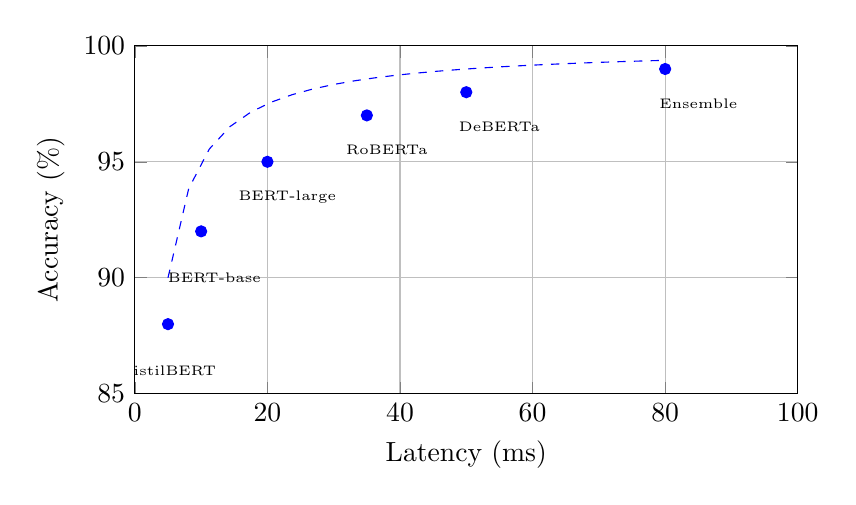
\begin{tikzpicture}
    \begin{axis}[
        xlabel={Latency (ms)},
        ylabel={Accuracy (\%)},
        xmin=0, xmax=100,
        ymin=85, ymax=100,
        legend pos=south east,
        width=10cm,
        height=6cm,
        grid=major
    ]
    % Example Pareto frontier
    \addplot[only marks, mark=*, blue] coordinates {
        (5, 88) (10, 92) (20, 95) (35, 97) (50, 98) (80, 99)
    };
    \addplot[dashed, blue, domain=5:80] {100 - 50/x};
    
    % Labels
    \node[font=\tiny] at (axis cs:5,86) {DistilBERT};
    \node[font=\tiny] at (axis cs:12,90) {BERT-base};
    \node[font=\tiny] at (axis cs:23,93.5) {BERT-large};
    \node[font=\tiny] at (axis cs:38,95.5) {RoBERTa};
    \node[font=\tiny] at (axis cs:55,96.5) {DeBERTa};
    \node[font=\tiny] at (axis cs:85,97.5) {Ensemble};
    \end{axis}
\end{tikzpicture}
\caption{Typical accuracy-latency Pareto frontier for NLP models.}
\end{figure}

\subsection{When to Use Smaller Models}

\begin{table}[H]
\centering
\caption{Model size decision factors}
\begin{tabularx}{\textwidth}{lXX}
\toprule
\textbf{Factor} & \textbf{Prefer Smaller} & \textbf{Prefer Larger} \\
\midrule
Latency requirement & < 50ms & Flexible \\
Deployment target & Edge, mobile & Server, cloud \\
Training data & Limited & Abundant \\
Task complexity & Simple/well-defined & Complex/open-ended \\
Budget & Constrained & Flexible \\
\bottomrule
\end{tabularx}
\end{table}

%==============================================================================
\section{Retrieval System Design}
\label{sec:retrieval_decision}
%==============================================================================

\subsection{Architecture by Scale}

\begin{figure}[H]
\centering
\begin{tikzpicture}[
    node distance=1.2cm,
    decision/.style={diamond, draw, aspect=2.5, inner sep=1pt, fill=lightyellow, font=\small},
    result/.style={rectangle, draw, rounded corners, fill=lightgreen, minimum width=3cm, font=\small, align=center},
    arrow/.style={->, thick}
]
    \node[decision] (scale) {Corpus size?};
    
    \node[result, below left=1.2cm and 1.5cm of scale] (small) {Cross-Encoder\\(compare all pairs)};
    \node[result, below=1.2cm of scale] (medium) {Two-Tower +\\Cross-Encoder rerank};
    \node[result, below right=1.2cm and 1.5cm of scale] (large) {Two-Tower + ANN +\\Multi-stage rerank};
    
    \draw[arrow] (scale) -- node[above, font=\tiny, sloped] {< 1K} (small);
    \draw[arrow] (scale) -- node[left, font=\tiny] {1K-1M} (medium);
    \draw[arrow] (scale) -- node[above, font=\tiny, sloped] {> 1M} (large);
\end{tikzpicture}
\caption{Retrieval architecture by corpus scale.}
\end{figure}

\subsection{Two-Stage Retrieval Design}

\begin{table}[H]
\centering
\caption{Two-stage retrieval configuration}
\begin{tabularx}{\textwidth}{lXX}
\toprule
\textbf{Aspect} & \textbf{Stage 1 (Retrieval)} & \textbf{Stage 2 (Reranking)} \\
\midrule
Model & Two-Tower (Dual Encoder) & Cross-Encoder \\
Metric to optimize & Recall@K & NDCG, MRR \\
Typical K & 100-1000 & 10-50 \\
Latency target & 1-10 ms & 20-100 ms \\
Compute per item & O(1) dot product & O(L²) attention \\
\bottomrule
\end{tabularx}
\end{table}

\subsection{ANN Algorithm Selection}

\begin{table}[H]
\centering
\caption{ANN algorithm selection guide}
\begin{tabularx}{\textwidth}{lXXX}
\toprule
\textbf{Algorithm} & \textbf{Best For} & \textbf{Trade-off} & \textbf{Memory} \\
\midrule
HNSW & Best recall & Slow index build & High \\
IVF-Flat & Balanced & Need more probes for recall & Medium \\
IVF-PQ & Large scale & Lower recall & Low \\
ScaNN & Production (Google) & Complex setup & Medium \\
\bottomrule
\end{tabularx}
\end{table}

%==============================================================================
\section{Common Trade-off Discussions}
\label{sec:tradeoffs}
%==============================================================================

\subsection{Accuracy vs. Latency}

\textbf{Techniques to improve latency while preserving accuracy}:
\begin{enumerate}
    \item \textbf{Quantization}: INT8 gives 2-4× speedup with < 1\% accuracy loss
    \item \textbf{Distillation}: Smaller student can retain 95-99\% of teacher quality
    \item \textbf{Pruning}: Structured pruning for real speedup
    \item \textbf{Caching}: Cache embeddings, predictions for repeated inputs
    \item \textbf{Early exit}: Stop processing when confident
\end{enumerate}

\begin{table}[H]
\centering
\caption{Latency reduction techniques}
\begin{tabularx}{\textwidth}{lXXX}
\toprule
\textbf{Technique} & \textbf{Speedup} & \textbf{Accuracy Impact} & \textbf{Complexity} \\
\midrule
INT8 quantization & 2-4× & < 1\% loss & Low \\
INT4 quantization & 4-8× & 1-3\% loss & Medium \\
Distillation & 2-10× & 1-5\% loss & Medium \\
Structured pruning & 2-4× & 1-3\% loss & Medium \\
Flash Attention & 2-4× & 0\% & Low \\
Speculative decoding & 2-3× & 0\% & Medium \\
\bottomrule
\end{tabularx}
\end{table}

\subsection{Training Cost vs. Inference Cost}

\textbf{When to invest in training}:
\begin{itemize}
    \item High inference volume amortizes training cost
    \item One-time training, many inference calls
    \item Training enables smaller inference model (distillation)
\end{itemize}

\textbf{When to minimize training}:
\begin{itemize}
    \item Rapid iteration needed
    \item Low inference volume
    \item Frequently changing requirements
\end{itemize}

\subsection{Model Complexity vs. Maintainability}

\begin{table}[H]
\centering
\caption{Complexity vs. maintainability trade-offs}
\begin{tabularx}{\textwidth}{lXX}
\toprule
\textbf{Aspect} & \textbf{Simple Model} & \textbf{Complex Model} \\
\midrule
Debugging & Easy & Hard \\
Iteration speed & Fast & Slow \\
Interpretability & High & Low \\
Peak performance & Lower & Higher \\
Team expertise needed & Lower & Higher \\
Production risk & Lower & Higher \\
\bottomrule
\end{tabularx}
\end{table}

\begin{keyinsight}[Start Simple, Add Complexity]
Always start with the simplest solution that could work:
\begin{enumerate}
    \item Baseline: Logistic regression / simple heuristics
    \item First ML: Gradient boosting for tabular, pretrained BERT for text
    \item Optimize: Custom architectures, ensemble, SOTA methods
\end{enumerate}
Add complexity only when simpler approaches fail to meet requirements.
\end{keyinsight}

\subsection{Generalization vs. Specialization}

\begin{table}[H]
\centering
\caption{General vs. specialized models}
\begin{tabularx}{\textwidth}{lXX}
\toprule
\textbf{Factor} & \textbf{General Model} & \textbf{Specialized Models} \\
\midrule
Number of models & 1 & N (per task/domain) \\
Maintenance & Easier & Harder \\
Per-task performance & Lower & Higher \\
Data efficiency & Can share data & Need task-specific data \\
Deployment & Simpler & More complex \\
When to use & Early stage, rapid iteration & Mature system, quality critical \\
\bottomrule
\end{tabularx}
\end{table}

%==============================================================================
\section{Debugging Decision Trees}
\label{sec:debugging_decisions}
%==============================================================================

\subsection{Model Not Learning}

\begin{figure}[H]
\centering
\begin{tikzpicture}[
    node distance=0.8cm,
    decision/.style={diamond, draw, aspect=3, inner sep=1pt, fill=lightyellow, font=\tiny},
    action/.style={rectangle, draw, rounded corners, fill=lightgreen, minimum width=2cm, font=\tiny, align=center},
    arrow/.style={->, thick}
]
    \node[decision] (start) {Loss decreasing?};
    
    \node[decision, below left=1cm and 1cm of start] (lr) {Tried different LR?};
    \node[decision, below right=1cm and 1cm of start] (overfit) {Overfitting?};
    
    \node[action, below left=0.8cm and 0cm of lr] (try_lr) {Try LR × 0.1\\and LR × 10};
    \node[decision, below right=0.8cm and 0cm of lr] (data) {Data correct?};
    
    \node[action, below left=0.8cm and 0cm of data] (check_data) {Visualize batches\\Check labels};
    \node[action, below right=0.8cm and 0cm of data] (bug) {Check model\\architecture};
    
    \node[action, below left=0.8cm and 0cm of overfit] (regularize) {Add regularization\\More data/augmentation};
    \node[action, below right=0.8cm and 0cm of overfit] (continue) {Continue training\\Monitor validation};
    
    \draw[arrow] (start) -- node[above, font=\tiny, sloped] {No} (lr);
    \draw[arrow] (start) -- node[above, font=\tiny, sloped] {Yes} (overfit);
    \draw[arrow] (lr) -- node[left, font=\tiny] {No} (try_lr);
    \draw[arrow] (lr) -- node[right, font=\tiny] {Yes} (data);
    \draw[arrow] (data) -- node[left, font=\tiny] {Unchecked} (check_data);
    \draw[arrow] (data) -- node[right, font=\tiny] {Correct} (bug);
    \draw[arrow] (overfit) -- node[left, font=\tiny] {Yes} (regularize);
    \draw[arrow] (overfit) -- node[right, font=\tiny] {No} (continue);
\end{tikzpicture}
\caption{Debugging decision tree: model not learning.}
\end{figure}

\subsection{Production Performance Degradation}

\begin{enumerate}
    \item \textbf{Check data pipeline}
    \begin{itemize}
        \item Feature distributions changed?
        \item Missing/null values increased?
        \item Data source changed?
    \end{itemize}
    
    \item \textbf{Check for data drift}
    \begin{itemize}
        \item Compare feature distributions over time
        \item PSI (Population Stability Index) > 0.25 indicates significant drift
    \end{itemize}
    
    \item \textbf{Segment analysis}
    \begin{itemize}
        \item Performance by user segment
        \item Performance by feature value ranges
        \item Identify affected subpopulations
    \end{itemize}
    
    \item \textbf{Model debugging}
    \begin{itemize}
        \item Feature importance analysis
        \item Error analysis on failing cases
        \item Compare to baseline/previous model
    \end{itemize}
\end{enumerate}

%==============================================================================
\section{Interview Question Patterns}
\label{sec:interview_patterns}
%==============================================================================

\subsection{System Design Questions}

\textbf{Common patterns}:
\begin{enumerate}
    \item Clarify requirements and constraints
    \item Propose high-level architecture
    \item Dive into ML components
    \item Discuss trade-offs
    \item Address scale and production concerns
\end{enumerate}

\begin{interviewq}
\textbf{Q: Design a content recommendation system for a news app.}

\textbf{Framework for answering}:

\textbf{1. Clarify}:
\begin{itemize}
    \item Scale: Users? Articles per day?
    \item Latency requirements?
    \item Cold start handling?
    \item Engagement metric to optimize?
\end{itemize}

\textbf{2. High-level architecture}:
\begin{itemize}
    \item Candidate generation: Fast retrieval of relevant articles
    \item Ranking: Score and order candidates
    \item Business logic: Diversity, freshness, etc.
\end{itemize}

\textbf{3. ML components}:
\begin{itemize}
    \item User tower: Encode user history and features
    \item Item tower: Encode article content and metadata
    \item Ranker: Cross-features, contextual signals
\end{itemize}

\textbf{4. Trade-offs}:
\begin{itemize}
    \item Two-tower vs. cross-encoder
    \item Real-time vs. batch personalization
    \item Exploration vs. exploitation
\end{itemize}

\textbf{5. Production concerns}:
\begin{itemize}
    \item A/B testing framework
    \item Feedback loops
    \item Monitoring for engagement metrics
\end{itemize}
\end{interviewq}

\subsection{Architecture Choice Questions}

\textbf{Pattern}: ``Would you use X or Y for this problem?''

\textbf{Framework}:
\begin{enumerate}
    \item State your choice clearly
    \item Explain the primary reason
    \item Acknowledge trade-offs
    \item Describe when you'd choose the alternative
\end{enumerate}

\begin{interviewq}
\textbf{Q: Would you use BERT or GPT for sentiment analysis?}

\textbf{A:} I would use \textbf{BERT} for the following reasons:

\textbf{Primary reason}: Sentiment analysis is a classification (understanding) task. BERT's bidirectional attention is better suited because sentiment often depends on context from both directions.

\textbf{Secondary reasons}:
\begin{itemize}
    \item Faster inference (no autoregressive decoding)
    \item More efficient fine-tuning for classification
    \item [CLS] token provides natural sentence representation
\end{itemize}

\textbf{Trade-offs}: GPT/LLMs could work via prompting without fine-tuning, which might be preferred if:
\begin{itemize}
    \item No labeled training data available
    \item Need zero-shot capability
    \item Want single model for multiple tasks
\end{itemize}
\end{interviewq}

\subsection{Trade-off Discussion Questions}

\textbf{Pattern}: ``How would you handle X constraint?''

\textbf{Framework}:
\begin{enumerate}
    \item Acknowledge the constraint explicitly
    \item List options with trade-offs
    \item Recommend based on typical scenarios
    \item Ask clarifying questions if needed
\end{enumerate}

\begin{interviewq}
\textbf{Q: Your model needs to run in < 10ms. Current latency is 50ms. What do you do?}

\textbf{A:} I'd approach this systematically:

\textbf{1. Profile to find bottleneck}:
\begin{itemize}
    \item Feature computation? → Pre-compute, cache
    \item Model forward pass? → Optimize model
    \item Post-processing? → Simplify logic
\end{itemize}

\textbf{2. Model optimization options} (in order of complexity):
\begin{itemize}
    \item \textbf{Quantization} (INT8): 2-4× speedup, minimal quality loss
    \item \textbf{Distillation}: Train smaller student model
    \item \textbf{Pruning}: Remove unnecessary weights
    \item \textbf{Architecture change}: Simpler model (e.g., DistilBERT vs BERT)
\end{itemize}

\textbf{3. System optimizations}:
\begin{itemize}
    \item Batching for throughput
    \item Better hardware (GPU, specialized accelerators)
    \item Caching frequent predictions
\end{itemize}

\textbf{My recommendation}: Start with INT8 quantization—it's low-effort and usually gets 3-4× speedup. If still not enough, distillation to a smaller model.
\end{interviewq}